% This is LLNCS.DOC the documentation file of
% the LaTeX2e class from Springer-Verlag
% for Lecture Notes in Computer Science, version 2.4
\documentclass{llncs}
\usepackage{llncsdoc}
\usepackage{graphicx}
\usepackage{amssymb}
\usepackage[table]{xcolor}
%\usepackage[cp1250]{inputenc} % WH
%\usepackage[polish]{babel}    % WH

% Added for code listing
\usepackage{listings}
\usepackage{caption}

\newcounter{nalg}[chapter] % defines algorithm counter for chapter-level
\renewcommand{\thenalg}{\thechapter .\arabic{nalg}} %defines appearance of the algorithm counter
\DeclareCaptionLabelFormat{algocaption}{Algorithm \thenalg} % defines a new caption label as Algorithm x.y

\lstnewenvironment{algorithm}[1][] %defines the algorithm listing environment
{
    \refstepcounter{nalg} %increments algorithm number
    \captionsetup{labelformat=algocaption,labelsep=colon} %defines the caption setup for: it ises label format as the declared caption label above and makes label and caption text to be separated by a ':'
    \lstset{ %this is the stype
        frame=tB,
        numbers=left,
        numberstyle=\tiny,
        basicstyle=\scriptsize,
        keywordstyle=\color{black}\bfseries\em,
        keywords={,input, output, return, datatype, function, in, if, else, foreach, while, begin, end, done, } %add the keywords you want, or load a language as Rubens explains in his comment above.
        numbers=left,
        xleftmargin=.04\textwidth,
        #1 % this is to add specific settings to an usage of this environment (for instnce, the caption and referable label)
    }
}
{}

\usepackage{url}
\urldef{\mailwhajwp}\path|{xxx,yyy,zzz}@mini.pw.edu.pl|
\newcommand{\keywords}[1]{\par\addvspace\baselineskip
\noindent\keywordname\enspace\ignorespaces#1}
%
\begin{document}


% first the title is needed
\title{Pattern Recognition with Rejection}
\subtitle{Combining Standard Classification Methods\\with Geometrical Rejecting}

% a short form should be given in case it is too long for the running head
\titlerunning{Pattern Recognition with Rejection}
%

\author{Wladyslaw Homenda\inst{1,2}, Agnieszka Jastrzebska\inst{1}, Piotr Waszkiewicz\inst{1}\\ and Anna Zawadzka\inst{1}}
%
\authorrunning{W. Homenda et. al}
% (feature abused for this document to repeat the title also on left hand pages)

% the affiliations are given next; don't give your e-mail address
% unless you accept that it will be published
\vspace{-6pt}
\institute{Faculty of Mathematics and Information Science, Warsaw University of Technology\\
ul. Koszykowa 75, 00-662 Warsaw, Poland \and Faculty of Economics and Informatics in Vilnius, University of Bialystok\\Kalvariju g. 135, LT-08221 Vilnius, Lithuania
}
\vspace{-6pt}
\maketitle
\vspace{-6pt}

\pagestyle{empty}  % no page numbers, no running headers

\begin{abstract}
\vspace{-12pt}
The motivation of our study is to provide algorithmic approaches to distinguish proper patterns, from garbage and erroneous patterns in pattern recognition problem. The design assumption is to provide methods based on proper patterns only. In this way the framework that we propose is truly versatile and it can be adapted to any pattern recognition problem in an uncertain environment, where garbage patterns may appear. The proposed attempt to recognition with rejection combines known classifiers with geometric methods used for separating native patterns from foreign ones. The proposed methods are empirically verified on datasets of handwritten digits classification (native patterns) and handwritten letters of Latin alphabet (foreign patterns).
\vspace{-6pt}
\keywords pattern recognition, classification, rejecting option, geometrical methods
\vspace{-6pt}
\end{abstract}


%\end{document}
\vspace{-12pt}
%-------------------------------------------------------------------
%-------------------------------------------------------------------
%-------------------------------------------------------------------
\section{Introduction}
  \label{sec:Introduction}
\vspace{-3pt}

The task of pattern recognition is a classical machine learning problem. On the input we pass a training dataset, consisting of labelled patterns belonging to $c$ classes. In the process we expect to form a model that would be able to assign correct labels to new patterns (new observations).

It is important to have in mind that patterns in their original form are some sort of signals, for instance images or voice recordings. Due to the fact that the original patterns are often collected using some signal-acquiring devices, we may encounter patterns that do not belong to any of proper classes. An example of such situation may happen, when the device that we use to acquire data has been automatically reset due to power outage and poor default calibration distorts the segmentation process. Another scenario may happen when we collect data in a noisy (out-of-lab) environment and apart from proper patterns there is a lot of unexpected residual elements. The problem with such patterns, say garbage patterns, is that we cannot predict their characteristic and therefore we cannot include information about them in the model training process.

The motivation of our study is to provide algorithmic approaches to distinguish proper patterns, that we call \textbf{native patterns} from garbage and erroneous patterns, that we call \textbf{foreign patterns}. The task that we describe we call \textbf{foreign patterns rejection}. The design assumption is to provide methods based on native patterns only. In this way the framework that we propose is truly versatile and it can be adapted to any pattern recognition problem in an uncertain environment, where foreign patterns may appear. 

In particular, the objectives of this paper are focused on designing methods for recognition with rejection and employ them to (a) distinguish native patterns from foreign ones and (b) improve classification quality of native patterns. The proposed attempt to recognition with rejection combines known classifiers with geometric methods used for separating native patterns from foreign ones. The proposed methods are empirically verified on datasets of handwritten digits (native patterns) and handwritten Latin letters (foreign patterns).

We would like to emphasis that the novelty of the contribution presented in this paper is not in the methods that we use, but in how we employ them and on what we achieve with them.
%TODO koniecznie trzeba dodac wiecej opisu novelty/objective, dodamy na koncu jak bedzie calosc artykulu

The remainder of this paper is organized as follows. Section \ref{sec:Literature Review} presents the background knowledge on foreign elements detection present in the literature. Sections~\ref{sec:Ellipsoids} and~\ref{sec:Classifiers} presents the backbone algorithms, known in the literature, that we use to construct our models. Section \ref{sec:Methodology} presents the proposed approach. In Section \ref{sec:Experiments} we discuss a series of experiments. % based on images of handwritten digits. 
Section \ref{sec:Conclusion} concludes the paper and highlights future research directions.
%Lastly, Section \ref{sec:Conclusion} concludes the paper and highlights future research directions.


\vspace{-3pt}
%-------------------------------------------------------------------
%-------------------------------------------------------------------
%-------------------------------------------------------------------
\section{Preliminaries}
  \label{sec:Preliminaries}
\vspace{-6pt}

Data collection and processing is a vital study problem across multiple domains of science. Along with a substantial automation of data acquiring we meet with difficulties that appear due to poor data quality. The research we present in this paper has been motivated by the issue of contaminated datasets, that apart from proper patterns contain garbage.

In this section we start discussion with review of relevant literature positions in machine learning that tackle the issue of contaminated datasets. Then, in order to provide a self-contained description of employed methods we present backbone literature algorithms applied. In what follows we present the Minimum Volume Enclosing Ellipsoid (MVEE) algorithm and a suite of 3 classification methods: Random Forests (RF), Support Vector Machines (SVM), and K-Nearest Neighbors algorithm (K-NN). Listed methods are employed in various configurations to native elements classification with foreign elements rejection. Our approach, based on those algorithms, is discussed in Section \ref{sec:Methodology}.


\vspace{-6pt}
%-------------------------------------------------------------------
%-------------------------------------------------------------------
\subsection{Literature Review}
  \label{sec:Literature Review}
\vspace{-3pt}

The rejecting option in pattern recognition problem has gained rather weak attention despite its importance in practice. Also, there is a~relatively short list of papers raising the problem of rejecting foreign patterns, cf.~\cite{HomendaICAART2015} for a~short survey.% In this paper we study several attempts to classification with rejection of foreign elements. Scenarios for the discussed methods is based on well-known combinations of machine learning algorithms.  
Here we only hint some issues present in literature neither with claiming to comprehensive coverage the subject, not giving deep background of methods employed in this study.

Discussion on approaches related to foreign elements rejection should also mention one-class classification methods. Especially, there are two noteworthy examples: centroid-based methods and One-Class Support Vector Machine.

Centroid-based methods rely on distinguishing cluster centres (centroids). Region reserved for proper elements is usually defined by the distance between centre and the furthest proper pattern.

One-Class SVM has been introduced in \cite{ScholkopfWilliamsonSmola1992}. While "regular" SVM algorithm forms hyperplane separating two classes, the One-Class SVM separates data points from the entire feature space. Notably, the One-Class SVM provides a soft decision rules, as there is a $\nu$ parameter determining the fraction for outliers.  

%It is worth to emphasize the analogy between outlier detection and foreign elements rejection. However, the motivation for those two problems remains different.

When it comes to the study on foreign elements rejection, there is relatively few papers to review. This issue, in spite of its importance, remains somehow neglected. Among noteworthy studies one may mention rank-based methods, for instance ones described in \cite{BertolamiZimmermannBunke2006,BurgerKessentiniPaquet2011,EladHel-OrKeshet2001,HempstalkFrankWitten2008,SchemeHudginsEnglehart2013,TaxDuin2008,WangCasasent2009}.
In a nutshell, mentioned papers propose to attach confidence scores along with class labels. Rejection occurs when none of native class labels was assigned with a satisfying confidence.

In our paper we assume an approach that in its background resembles more model-based outlier detection techniques than reported in the literature foreign elements rejection schemes. The objective of our study is to form a model that would be able to distinguish between the region reserved for native patterns and the remainder of the feature space. 

%-------------------------------------------------------------------
%-------------------------------------------------------------------
%\subsection{Backbone Algorithms}
%  \label{sec:BackboneAlgorithms}

\vspace{-6pt}
%-------------------------------------------------------------------
%-------------------------------------------------------------------
\subsection{Ellipsoids for Foreign Elements Rejection}
  \label{sec:Ellipsoids}
\vspace{-3pt}

%description of the idea of geometrical rejection
%issues: location, size, parameters of those figures

% Links used in this description
% Link: http://geomalgorithms.com/a08-_containers.html
% http://people.orie.cornell.edu/miketodd/TYKhach.pdf
Both native and foreign patterns are represented by certain vector of features extracted from pattern of interest. Features are usually represented as real numbers, therefore every pattern is a point in multidimensional Euclidean space. What's more, if it turned out that the sets of those points representing symbols, each forms a tight cluster in space, it might be possible to find their respective minimal enclosing boxes.

In computational geometry, the smallest enclosing box problem is that of finding the oriented minimum bounding box enclosing a~set of points. As opposed to convex hull, which is the most accurate point set container with smallest volume and which is enclosed by linear hyper planes. Bounding boxes are far less complex. In many cases, when there's a need for computing convex hull and testing inclusions of other points, an approximation of such hull can be used, which helps to reduce time needed for computations, since most of alternative methods have lower construction and inclusion-testing complexities. Some of such approaches include using figures like hypercubes, diamonds, spheres or ellipsoids to successfully enclose given set of points.

When comparing highlights and drawbacks of each method, from computational complexity perspective, ease of testing point inclusion and algorithm implementation point of view, ellipsoids seem to be a reasonable choice. Constructed ellipsoid is superior to the minimal cuboid in many ways. It is unique, gives better approximation of the object it contains and if $E(S)$ is the bounding ellipsoid for a point set $S$ with convex hull $C(S)$ in dimension \textit{d}, then:

\[ 
  \frac{1}{d}E(S) \subseteq C(S) \subseteq E(S) 
\]
where scaling is with respect to the center of $E(S)$.

Adaptation of the smallest enclosing box problem to foreign elements rejection, or native elements identification, seems to be a very natural approach. The justification is fairly simple: if we enclose elements belonging to native classes, using for instance ellipsoids, formed geometrical model will discriminate a region of the features space reserved for native patterns between a region where we may encounter foreign patterns. With this premise in mind, let us present a detailed description of the MVEE algorithm.

\vspace{-9pt}
%-------------------------------------------------------------------
\subsubsection{MVEE}

% Links used:
% http://citeseerx.ist.psu.edu/viewdoc/download;jsessionid=3A12C2006473A250D78C45B99B0BB3FA?doi=10.1.1.116.7691&rep=rep1&type=pdf
% http://www.mathworks.com/matlabcentral/fileexchange/9542-minimum-volume-enclosing-ellipsoid/content/MinVolEllipse.m
% http://stackoverflow.com/questions/1768197/bounding-ellipse/1768440#1768440
% http://stackoverflow.com/questions/14016898/port-matlab-bounding-ellipsoid-code-to-python

problem is solved by several known algorithms that can be categorized as first-order, second-order interior-point or combination of the two. For small dimensions \textit{d}, the MVEE problem can be solved in \textit{O($d^{O(d)}$m)} operations using randomized or deterministic algorithms~\cite{MVEEMichaelTodd2005}. In this paper the algorithm based on Khachiyan solution is used.

\noindent An ellipsoid in center form is given by 
\[ 
  E = \{x \in \mathbb{R}^{n} | (x - c)^{T}A(x-c) \le 1\} 
\] 
where $c \in \mathbb{R}^{n}$ is the center of the ellipse E and $ A \in \mathbb{S}^{n}_{++}$. Points lying inside the ellipse satisfy 
\[ 
  (x_{i} - c)^{T}A(x_{i} - c) \le 1 + acceptance 
\] 
where acceptance parameter defines the error margin in determining point belonging to ellipsoid, i.e. it alows to enlarge the ellipsoid.% It can be imagined as testing point inclusion on enlarged ellipsoid.

However, presented equation, is not a convex optimization problem and it has to be changed. It turns out that even then, the solution is not easily obtainable so the dual problem has to be found. For more precise and in depth solution description see \cite{MVEEMichaelTodd2005}. The main problem, when using ellipsoids as identifiers, lies in constructing them. Two main factors that decide about identification effectiveness are tolerance and acceptance parameters. Tolerance can be viewed as a threshold for ellipsoid construction accuracy. The lower the parameter is, the better minimal volume ellipsoid is created. On the other hand, even with good training set, there's a risk of including native elements that lie outside of created ellipsoid. To prevent such unwanted behaviour acceptance has been introduced. It defines threshold for point rejection for points lying outside of created figure.  

\vspace{-6pt}
%-------------------------------------------------------------------
%-------------------------------------------------------------------
\subsection{Native Elements Classification}
  \label{sec:Classifiers}
\vspace{-3pt}

The task of native elements classification relies on forming a model based on a labelled training dataset that assigns proper class labels to new problem instances. In a conventional scenario the training dataset consists of $m$ instances of $n$-dimensional feature vectors. Feature vectors are numerical descriptors of actual patterns. There is a multitude of classification algorithms, among which we have selected 3 different ones that are applied in our methods. It is necessary to emphasize that if someone would like to adapt our method to their own domain, those algorithms could be substituted with some other classification tools that may be more efficient in that domain. Without further ado let us move towards a brief description of the methods that we apply in our study.

\vspace{-9pt}
%-------------------------------------------------------------------
\subsubsection{Support Vector Machines}

% Used links:
% http://scikit-learn.org/stable/modules/svm.html#svm-kernels
are a set of supervised learning methods used for classification, regression and outliers detection. The SVM algorithm relies on a construction of hyperplane with a maximal margin that separates instances of two classes, \cite{CortesVapnik1995}. SVMs are effective in high dimensional spaces, memory efficient and quite versatile with many kernel functions that can be specified for the decision function. Although in some cases, where number of features is much greater than the number of samples, this method can give poor results, and is not cost-efficient when calculating probability estimates, it is well suited for problem presented in this paper. Given a set of training examples, each marked for belonging to one of two categories, an SVM training algorithm builds a model that assigns new examples into one category or the another. For multi-class classification "one-against-one" approach is used. For \textit{n} classes \textit{n} * (\textit{n} - 1) / 2 classifiers are constructed, each one is trained with data from two different classes. In our study we use decimal digits as classes. Therefore, the following 45 class-against-class SVMs are built: "0 vs 1", "0 vs 2", \dots "0 vs \textit{9}", "1 vs 2", \dots "1 vs 9",  \dots "\textit{8} vs \textit{9}". Classification decision is taken by voting method, i.e. a new pattern subjected to classification is counted to the most frequent class among these 45 binary classifiers. The case when two or more classes are most frequent, a second choice decision is made for actual classification. For instance, the closest pattern from most popular classes or minimal sum of distances from the processed pattern to ones from most popular classes may decide.  

\vspace{-9pt}
%-------------------------------------------------------------------
\subsubsection{Random Forests}

is a popular ensemble method. The main principle behind ensemble methods, in general, is that a group of "weak learners" can come together to form a "strong learner". In the Random Forests algorithm the weak learners are decision trees, which are used to predict the membership of objects in the classes. For vector of independent variables representing one object they calculate the value of the class the object belongs to by dividing value space into two or more subspaces. More precisely, an input data is entered at the top of the tree and as it traverses down the tree the data gets bucketed into smaller and smaller sets. In this method a large number of classification trees is generated. To grow each tree a random selection with replacement is made from the examples in the training set $D$. Those subsets $D_{k}$ are called bootstrap training sets. At each node $m$ variables are selected at random out of the set of input variables and the best split on these $m$ is used to split the node. After a relatively large number of trees is generated, they vote for the most popular class. Random Forests join few important benefits: (a) they are relatively prone to the influence of outliers, (b) they have an embedded ability of feature selection, (c) they are prone to missing values, and (d) they are prone to overfitting, \cite{Breiman2001}. 

\vspace{-9pt}
%-------------------------------------------------------------------
\subsubsection{K-Nearest Neighbors}

is an example of a "lazy classifier", where the entire training dataset is a model. There is no typical model building phase, hence the name. Class membership is determined based on class labels encountered in K closest observations in the training dataset, \cite{Altman1992}. In a typical application, the only choices the model designer has to make are selection of K and distance metrics. Both are often extracted with a help of a supervised learning procedures.
%TODO te opisy mozna rozszerzyc - czy dodac to potem zdecydujemy

%-------------------------------------------------------------------
%-------------------------------------------------------------------
%-------------------------------------------------------------------
\section{Methodology}
  \label{sec:Methodology}
  
There are two approaches used to determine whether an object is rejected (classified as foreign). First one assumes the use of classification methods, which originally were not designed for elements rejection. The second approach involves using classifiers as the only classification tool, whereas rejecting is realized by ellipsoids. In this section let us present the second approach to foreign elements rejection.

%-------------------------------------------------------------------
%-------------------------------------------------------------------
\subsection{External Global and Local Rejecting}
  \label{subsec:GlobalLocalRejecting}

Whereas ellipsoids are good identifiers, they lack in element classification quality. This is caused by the fact that ellipsoids may overlap each other, which results in points belonging to both classes at the same time. Although this can be solved by calculating distance between those elements and each ellipsoid centre, or taking value of ellipsoid-inclusion equation as a classification measure, tests have proven that such approaches are more prone to errors than other classifiers mentioned in this paper. Taking into considerations both strengths and weaknesses of classifiers and identifiers, the combined solution has been prepared that employs both tools (classifiers and ellipsoids), making use of their advantages.

Classifiers have high success rate but cannot distinguish between foreign elements and native ones. Contrary to that, ellipsoids tend to be better at rejecting foreign patterns, which makes them good at identifying points that should not be classified. The natural way of dealing with that problem would be to use ellipsoids as first-entry identifier that purifies input set by removing foreig patterns. The result of such rejection would be sent to the chosen classifier that would classify remaining native elements. Schema of this method is presented on the left part of Figure~\ref{fig:nativeforeignpatternsClassification1}


\begin{figure}[!h]
  \centering
  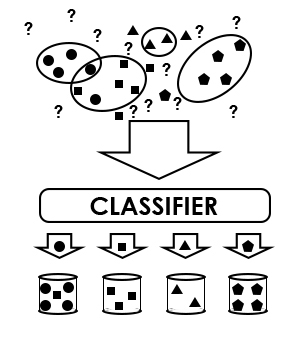
\includegraphics[width=0.47\textwidth]{_Figures/Classification1.jpg}\hspace{12pt}
	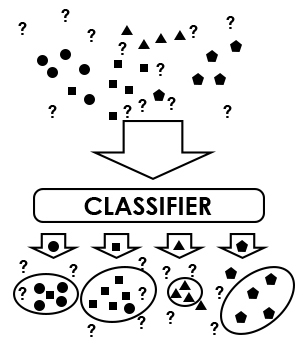
\includegraphics[width=0.47\textwidth]{_Figures/Classification2.jpg}
  \caption{Recognition with ellipsoids employed for rejecting: ellipsoids as identifiers reject foreign elements (left part) and ellipsoids as correctors (right part)}
\label{fig:nativeforeignpatternsClassification1}
\end{figure}

Another way of using ellipsoids as identifiers is to treat them as correctors. That means there's no need to remove foreign elements from the set before classification, as rejection is done later. After all elements have been classified, identification for each class is done by using class-corresponding ellipsoid. There's a possibility that some foreign elements will be assigned to a class with a corresponding ellipsoid that will reject them. This is somewhat different from previous approach because elements can be rejected even if there is an ellipsoid that would pass inclusion test. The schema can be seen on the right part of Figure~\ref{fig:nativeforeignpatternsClassification1}

%\begin{figure}[!h]
%	\centering
%	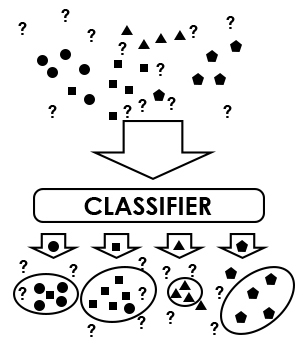
\includegraphics[width=0.5\textwidth]{_Figures/Classification2.jpg}
%	\caption{Ellipsoids as correctors. Classifiers try to classify foreign elements that will be rejected later}
%	\label{fig:nativeforeignpatternsClassification2}
%\end{figure}


%-------------------------------------------------------------------
%-------------------------------------------------------------------
\subsection{Quality Evaluation}

In order to evaluate the quality of proposed methods the patterns from the following groups are counted:
\begin{itemize}
\item CC  (Correctly Classified) - correctly classified patterns, i.e. native patterns classified as native ones with the correct class,
\item TP  (True Positives) - native patterns classified as native (no matter, into which native class),
\item FN  (False Negatives) - native patterns incorrectly classified as foreign,
\item FP  (False Positives) - foreign patterns incorrectly classified as native,
\item TN  (True Negatives) - foreign patterns correctly classified as foreign.
\end{itemize}
These numbers are then used to form measures reflecting specific aspects of classification and rejection, cf. Table~\ref{tab:measures}. Notions that we use are well-known in the domain of pattern recognition. We have included a detailed description of those measures in our previous paper \cite{HomendaICAART2015}.
\begin{table}[!htbp]
\centering
\caption{Quality measures for classification and rejection}
{\footnotesize
\begin{tabular}{rclrcl}
  $\textnormal{Native Precision}$ &$=$& $\displaystyle\frac{\textnormal{TP}}{\textnormal{TP+FP}}$ & 
  $\textnormal{Accuracy}$ &$=$& $\displaystyle\frac{\textnormal{TP+TN}}{\textnormal{TP+FN+FP+TN}}$ \\
  &&&&&\vspace{-3pt}\\
  $\textnormal{Foreign Precision}$ &$=$& $\displaystyle\frac{\textnormal{TN}}{\textnormal{TN+FN}}$ &
  $\textnormal{Strict Accuracy}$ &$=$& $\displaystyle\frac{\textnormal{CC+TN}}{\textnormal{TP+FN+FP+TN}}$ \\
  &&&&&\vspace{-3pt}\\
  $\textnormal{Native Sensitivity}$ &$=$& $\displaystyle\frac{\textnormal{TP}}{\textnormal{TP+FN}}$ &
  $\textnormal{Fine Accuracy}$ &$=$& $\displaystyle\frac{\textnormal{CC}}{\textnormal{TP}}$ \\
  &&&&&\vspace{-3pt}\\
  $\textnormal{Foreign Sensitivity}$ &$=$& $\displaystyle\frac{\textnormal{TN}}{\textnormal{TN+FP}}$ &
  $\hspace{18pt}\textnormal{Strict Native Senssitivity}$ &$=$& $\displaystyle\frac{\textnormal{CC}}{\textnormal{TP+FN}}$\\
  &&&&&\vspace{-3pt}\\
  \multicolumn{6}{c}{$\textnormal{F--measure}=2\cdot\displaystyle\frac{\textnormal{Precision}\cdot\textnormal{Sensitivity}}{\textnormal{Precision}+\textnormal{Sensitivity}}$}\\
\end{tabular}
}
\label{tab:measures}
\vspace{-6pt}
\end{table}

\begin{itemize}
  \item \emph{Strict Accuracy} measures classifier's performance. It is the ratio of the number of all \emph{correctly classified} patterns to the number of all patterns being processed.
  \item \emph{Accuracy} is a "softer" characteristic derived from the Strict Accuracy. Accuracy describes the ability to distinguish between native and foreign patterns. The difference is that we do not require that the native patterns are labelled with their proper class label.
  \item \emph{Native Precision} is the ratio of the number of not rejected native patterns to the number of all not rejected patterns (i.e. all not rejected native and foreign ones). The higher the value of this measure, the better ability to distinguish foreign elements from native ones. Native Precision does not evaluate how effective identification of native elements is.
  \item \emph{Native Sensitivity} is the ratio of the number of not rejected native patterns to all native ones. The higher the value of Native Sensitivity, the more effective identification of native elements. Unlike the Native Precision, this measure does not evaluate the effectiveness of separation between native and foreign elements.
  \item \emph{Strict Native Sensitivity} takes only correctly classified native patterns and does not consider native patterns, which are not rejected and assigned to incorrect classes, unlike Native Sensitivity, where all not rejected native patterns are taken into account.
  \item \emph{Fine Accuracy} is the ratio of the number of native patterns classified to correct classes, i.e. assigned to their respective classes, to the number of all native patterns not rejected. This measure conveys how precise is correct classification of not rejected patterns.
  \item \emph{Foreign Precision} corresponds to Native Precision.
  \item \emph{Foreign Sensitivity} corresponds to Native Sensitivity.
  \item  Precision and Sensitivity are complementary and there exists yet another characteristic that combines them: the \textit{F--measure}. It is there to express the balance between precision and sensitivity since these two measures affect each other. Increasing sensitivity can cause a~drop in precision since, along with correctly classified elements, there might be more incorrectly classified.
\end{itemize}


%-------------------------------------------------------------------
%-------------------------------------------------------------------
%-------------------------------------------------------------------
\section{Experiments}
  \label{sec:Experiments}

In this section we move towards description of a series of experiments where we apply rejection strategies discussed theoretically in Sections~\ref{subsec:GlobalLocalRejecting}. In what follows we describe the datasets, experiments' settings and the results. 

%-------------------------------------------------------------------
%-------------------------------------------------------------------
\subsection{Datasets}

The Experiments' section is devoted to a study on handwritten digits recognition and handwritten letters rejection. 

Foreign patterns are usually unknown. In this study as foreign patterns we assume a dataset of handwritten letters from the Latin alphabet. The justification to assume such foreign dataset for testing purposes is that appearance of other real symbols, not belonging to any proper class, is a common issue in a character recognition problem. 

We would like to stress again, that foreign patterns do not participate in model building phase. The entire scheme is based on native patterns only. Handwritten letters are used only for rejection mechanisms quality evaluation. Samples of processed patterns are displayed in Figure \ref{fig:nativeforeignpatterns}.

\begin{figure}[!tbp]
\vspace{-6pt}
  \centering
  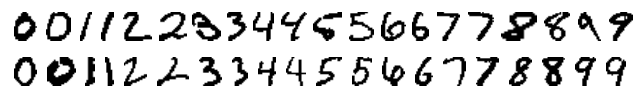
\includegraphics[width=0.49\textwidth]{_Figures/natives}\\
  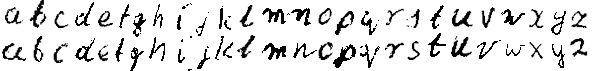
\includegraphics[width=0.7\textwidth]{_Figures/foreigns}
\vspace{-6pt}
  \caption{Sample of: native patterns (top) and foreign patterns (bottom).}
\label{fig:nativeforeignpatterns}
\vspace{-12pt}
\end{figure}

The training dataset was made of 10,000 handwritten digits with approximately 1,000 observations in each class taken from publicly available MNIST database, \cite{LeCunCortesBurges}. We split each class in proportion ca. 7:3 and in a process we got two sets. The first one includes 6,996 patterns and is used for training. The second set, the test set, contains 3,004 patterns. The dataset of foreign patterns contains 26,383 handwritten Latin letters, ca. 1,000 letters in each class. This dataset was created by 16 students, writing about 70 copies of each letter.

All patterns were normalized and feature vectors comprising of 106 numerical features were created. Examples of features are: maximum/position of maximum values of projections, histograms of projections, transitions, offsets; raw moments, central moments, Euler numbers etc.  The best first search for the optimal feature subset has been performed using FSelector R package, \cite{Romanski} and then ANOVA was employed to select independent features. The final feature vector contained 24 features. We considered features standardization but the training data is sufficiently consistent (there is no outliers), so we normalized those features to bring linearly all values into the range [0,1]. 

%Best first search is one of popular wrapper feature selection methods. Wrapper methods select multiple subsets of features, for all those subsets they train a classifier (in general: a model) and they select this subset for which numerical quality was the best. In our particular case as quality evaluator we used a 10-class SVM. A commonly known advantage of wrapper feature selection methods is that the subsets they select usually provide satisfying performance. The disadvantage is their computational complexity. The best first search for the optimal feature subset has been performed using FSelector R package, \cite{Romanski}. The final feature vector contained 24 features. We considered features standardization but the training data is sufficiently consistent (there is no outliers), so we normalized those features to bring linearly all values into the range [0,1].
%\begin{equation}\label{eqn:normalization}
%    X'_{i,j} = \frac{X_{i,j} - Min_{j}}{Max_{j}-Min_{j}}
%\end{equation}
%where $X_{i,j}$ is the value of $j^{th}$ feature in $i^{th}$ observation, $Min_{j}$ and $Max_{j}$ are respectively the minimum and maxium value of $j^{th}$ feature.


\vspace{-6pt}
%-------------------------------------------------------------------
%-------------------------------------------------------------------
\subsection{Experimental Settings}
\vspace{-3pt}

Solutions presented in this paper has been implemented in Python programming language, using scientific libraries \cite{MatLab,NumPy,Scikit}. %- NumPy\footnote{NumPy website: http://www.numpy.org/}, Scikit\footnote{Scikit website: http://scikit-learn.org/stable/}. Implementations of classifiers described in this article have been imported from Scikit library \cite{Scikit}
%{ScikitSVM,ScikitRF,ScikitKNN}.\\
The MVEE algorithm, available as MATLAB code \footnote{http://www.mathworks.com/matlabcentral/fileexchange/9542-minimum-volume-enclosing-ellipsoid/content/MinVolEllipse.m} has been rewritten in Python language, using NumPy library for matrix representation and operations. Several tests have been performed in order to find best suited method parameters for both classifiers and identifiers. For finding those values the Grid Search~\cite{Scikit} %\footnote{Link to Python implementation: http://scikit-learn.org/stable/modules/grid\_search.html} 
has been used for SVM and Random Forests. Ellipsoids and KNN methods had their values assigned manually. 

\vspace{-6pt}
%-------------------------------------------------------------------
\subsubsection{MVEE method parameters}
Each ellipsoid was created and used with two parameters: tolerance and acceptance. The tolerance argument was used during creation phase, as "accuracy measurement". Lower value means that created enclosing figure is more fitted to the construction set. Acceptance parameter defines how far can point lie outside the ellipsoid to still be identified as belonging to it. In other words, it treats enclosing ellipsoid as being bigger than it really is.
Parameters tests involved computing effectiveness of MVEE algorithm for certain tolerance and acceptance values. We tested values from such ranges:\vspace{-6pt}
\begin{itemize}
	\item tolerance = [0.5, 0.2, 0.1, 0.01]
	\item accuracy = [0.1, 0.01, 0.001, 0.0005]
\end{itemize} 
The results revealed that for given training and test sets the best parameter combination was tolerance=0.5 and accuracy=0.1 and those values were used in final, combined method described later in this document.

\vspace{-6pt}
%-------------------------------------------------------------------
\subsubsection{SVM method parameters}
SVM method available in Scikit package offers a few built-in kernels that were used during computations: radial basis function and polynomial. Additionally, there are two more parameters that were tested: C (described as penalty parameter C of the error term), and $\gamma$ (known as kernel coefficient). Values that were tested:\vspace{-6pt}
\begin{itemize}
	\item kernel = ['rbf', 'poly']
	\item C = [1, 2, 4, 5, 16]
	\item $\gamma = [2^{-1}, 2^{-2}, 2^{-3}, 0,00025]$
\end{itemize}
The best found combination of those parameters used rbf kernel along with C=8 and $\gamma = 2^{-1}$ values.

\vspace{-6pt}
%-------------------------------------------------------------------
\subsubsection{Random Forests method parameters}
Scikit library was used to test random forests. Random forests with the following number of trees were tested: 1, 2, 3, 5, 10, 20, 30, 40, 50, 60, 70, 80, 90, 100, 110, 120, 130, 140, 150. The best number of trees to build the forest is 100.

\vspace{-6pt}
%-------------------------------------------------------------------
\subsubsection{KNN method parameters}
The package was used for the k-NN classifier testing. We tested values of K (number of neighbors) such as: 1, 2, 3, 4, 5, 10, 20, 30, 40, 50. The best found value of k is 4. There is also one parameter - metric, but we use default value, which is standard Euclidean metric.


%-------------------------------------------------------------------
%-------------------------------------------------------------------
%\subsection{Concept of Classification with Rejection}
\subsection{Results of Experiments}
  \label{subsec:ClassificationAndRejection}

To determine effectiveness of parameter values for each method, confusion matrix has been calculated. Each row of this matrix represents information about distribution of patterns from certain class. For instance, 213 zeros were correctly classified to their class, 4 zeros were incorrectly classified as ones, 2 zeros - as sixes, 17 zeros as eights and 58 zeros were incorrectly rejected as non-digit patters, cf. row "0" in Table~\ref{tab:CofusionTable}. Numbers in each column hold information about quantity of patterns that were classified as belonging to the corresponding class.

\begin{table*}[h]
\centering
\caption{Confusion table, data taken from ... }
\vspace{-3pt}
\setlength{\tabcolsep}{3pt}
\renewcommand{\arraystretch}{1}
{\footnotesize
\begin{tabular}{|c||r|r|r|r|r|r|r|r|r|r|r|}
\hline
 \hspace{15pt} & $0\;\;\;$ & $1\;\;\;$ & $2\;\;\;$ & $3\;\;\;$ & $4\;\;\;$ & $5\;\;\;$ & $6\;\;\;$ & $7\;\;\;$ & $8\;\;\;$ & $9\;\;\;$ & $f$ \\
\hline\hline
  0 & 213 & 4 &   &   &   &   & 2 &   & 17 &   & 58\\
\hline
  1 &  & 259 & 1 &   &   &   &   &   &   &   & 81\\
\hline
  2 &  &   & 227 &   &   &   &   &   &   &   & 83\\
\hline
  3 &  &   &   & 206 &   & 4 &   & 2 & 2 &   & 89\\
\hline
  4 &  &   &   &   & 202 &   &   & 2 & 1 & 2 & 88\\
\hline
  5 &  &   &   & 5 & 1 & 189 &   &   & 2 &   & 71\\
\hline
  6 &  & 1 &   &   &   &   & 219 &   & 1 &   & 67\\
\hline
  7 &  &   & 1 &   & 1 &   &   & 243 &   & 1 & 63\\
\hline
  8 & 1 &   &   &   & 1 &   &   &   & 213 &   & 78\\
\hline
  9 &  &   &   &   & 6 & 1 &   & 6 & 2 & 230 & 58\\
\hline
$f$ & 66 & 20 & 48 &   & 110  & 16 & 54 & 1 & 126 & 15 & 25927\\
\hline
\end{tabular}
}
\vspace{-3pt}
\label{tab:CofusionTable}
\end{table*}
% TODO: Zmienić na "właściwe" wyniki: SVM external global rejection

Calculations and measurements included in "Quality Evaluation" section were based on confusion matrixes. Information gathered from them will be used in the following sections of this paper. The most interesting aspects of it consist of classification quality, rejection quality and rejection impact on classification quality. Those issues are the main and most important part of problem described in this paper.

%-------------------------------------------------------------------
\subsubsection{Influence of Rejection on Native Patterns Classification}

%ideally rejection improves classification by rejecting those element that would have been incorrectly classified

\begin{table}[h]
\centering
\caption{Results for classification with rejection on train and test sets of native patterns in comparison with classification results without rejection mechanism. RF - results for random forest, SVM - results for Support Vector Machines
%, .... \color{red}W ponizszej tabelce beda dane dotyczace odrzucania tylko na natives za pomoc� elipsoid i na dwoch poziomach (global i local). Czy jest sens dla train set? Czy nie bedzie 100\%? Na poziomie local chyba nie bedzie 100\%, dlatego jest sens. {\color{blue}Jako ostatnie dodane jest internal rejecting - czy dajemy te wyniki?} 
}
%\vspace{3pt}
\setlength{\tabcolsep}{3pt}
\renewcommand{\arraystretch}{1}
{\footnotesize
\begin{tabular}{|r||c|c|c||c|c|c||c|c|c|}
\hline
& \multicolumn{3}{c||}{No rejection} & \multicolumn{3}{c||}{Global rejection} & \multicolumn{3}{c|}{Local rejection}\\
\hline
  Basic Classifier & $\;\;$RF$\;\;$ & $\,$SVM$\,$ & KNN & $\;\;$RF$\;\;$ & $\,$SVM$\,$ & KNN & $\;\;$RF$\;\;$ & $\,$SVM$\,$ & KNN  \\
  \hline
  Data Set & \multicolumn{9}{c|}{Native Patterns, Train Set} \\
\hline
Fine Accuracy       & $1$ & $0.985$ & $0.955$ & $1$     & $0.987$ & $0.972$ & $1$ & $0.989$ & $0.984$ \\
Strict Native Sens. & $1$ & $0.985$ & $0.955$ & $0.879$ & $0.852$ & $0.854$ & $0.864$ & $0.857$ & $0.845$ \\
Native Sensitivity  & $1$ & $0.985$ & $0.955$ & $0.879$ & $0.879$ & $0.879$ & $0.864$ & $0.867$ & $0.859$ \\
\hline
  Data Set & \multicolumn{9}{c|}{Native Patterns, Test Set} \\
\hline
Fine Accuracy       & $0.952$ & $0.966$ & $0.930$ & $0.972$ & $0.982$ & $0.959$ & $0.977$ & $0.985$ & $0.976$ \\
Strict Native Sens. & $0.952$ & $0.966$ & $0.930$ & $0.842$ & $0.852$ & $0.831$ & $0.837$ & $0.845$ & $0.825$ \\
Native Sensitivity  & $0.952$ & $0.966$ & $0.930$ & $0.867$ & $0.867$ & $0.867$ & $0.857$ & $0.858$ & $0.845$ \\
\hline
\end{tabular}
}

% TODO: Poprawić tabelkę
% To co ma CC w liczniku
% Strict native 

\vspace{-6pt}
\label{tab:NativeNoForeign}
\end{table}

Adding a~rejection mechanism, ideally, may be seen as a~method for improvement of classification rates. It would be perceived as a~positive side of the rejection mechanism, if it would be able to reject those native patterns, which would be incorrectly classified when there is no rejection mechanism at all. Trained models only partially fulfil this wish. Conducted tests show that performing element rejection after their initial classification (local rejection scheme), brings better results. This could be explained by the fact that in the local rejection scheme we use one ellipsoid per each class and we apply those ellipsoids after classification. In contrast, in the global scheme we have a~joint set of ellipsoids that we apply to the entire dataset. In the local rejection scenario native elements identification regions are applied individually to each subset obtained from the classifier. As a result there is a chance that classification would contribute to foreign elements filtration. The same conclusion, about superiority of local rejection over global one concerns strict classification error ratios.

%-------------------------------------------------------------------
%-------------------------------------------------------------------
\subsection{Separating Letters from Digits}

Figure \ref{fig:Measures} presents rejection results. We compare various quality measures for models constructed based on random forest, SVM, and kNN with ellipsoids. 

Results show that all classifiers behave well and provide similar quality of rejection.   

\begin{figure}[!htbp]
  \centering
  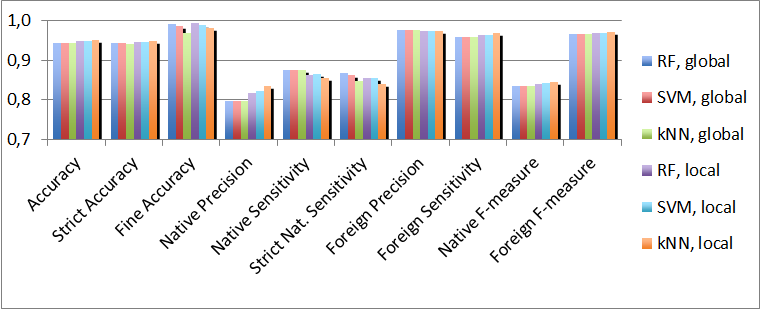
\includegraphics[width=\textwidth]{_Figures/Measures}\\
  \caption{Sample of: native patterns (top) and foreign patterns (bottom).}
\label{fig:Measures}
\vspace{-6pt}
\end{figure}

%TODO: na razie wlasciwe wyniki sa w 2 tabelkach, czesciowo sie powtarzaja, jak tabelki zostana uzupelnione bedziemy myslec o atrakcyjniejszym przedstawieniu wynikow (wykresy)}


%-------------------------------------------------------------------
%-------------------------------------------------------------------
%\subsection{MVEE Parameters and their Influence on Rejection Quality}


%\vfill
%\pagebreak
%-------------------------------------------------------------------
%-------------------------------------------------------------------
%-------------------------------------------------------------------
\section{Conclusion}
  \label{sec:Conclusion}

% TODO: Testy przeprowadzone, odpowiedzieć na pytanie czy współpraca jest zadowalająca, wpływ na rozpoznawanie native, zestaw danych zbyt ubogi?

Proposed ...


In future ....

Let us conclude this paper by saying that various adaptations of the idea of foreign elements rejection have a vital role in modern machine learning. It is needless to mention areas such as text mining, fraud detection, or medical diagnosis systems where we deal with various reincarnations of the foreign elements. In this perspective we believe that the study in this direction is worth further efforts.

%-------------------------------------------------------------------
%-------------------------------------------------------------------
%-------------------------------------------------------------------

\section*{Acknowledgment}

\noindent The research is partially supported  by the National Science Center, grant No 2012/07/B/ST6/01501, decision no \mbox{DEC-2012/07/B/ST6/01501}.


%-------------------------------------------------------------------
%-------------------------------------------------------------------
%-------------------------------------------------------------------
\begin{thebibliography}{1}

\bibitem{Altman1992}
Altman N. S., \emph{An introduction to kernel and nearest-neighbor nonparametric regression}. The American Statistician 46 (3), 1992, pp. 175-185.

\bibitem{BertolamiZimmermannBunke2006}
Bertolami R., Zimmermann M., Bunke H., \emph{Rejection strategies for offline handwritten text line recognition}, Pattern Recognition Letters 27(16), 2006, pp. 2005-2012.

\bibitem{Breiman2001}
Breiman L., \emph{Random Forests}. Machine Learning 45 (1), 2001, pp. 5�32. 

\bibitem{BurgerKessentiniPaquet2011}
Burger T., Kessentini Y., Paquet T., \emph{Dempster-Shafer based rejection strategy for handwritten word recognition}, Proc. of the 2011 International Conference on Document Analysis and Recognition, 2011, pp. 528-532.

\bibitem{CortesVapnik1995}
Cortes C., Vapnik V., \emph{Support-vector networks}. Machine Learning 20 (3), 1995, pp. 273-297.
 
\bibitem{EladHel-OrKeshet2001}
Elad M., Hel-Or Y., Keshet R., \emph{Pattern detection using maximal rejection classiffier}, C. Arcelli et al. (Eds.): Proc. International Workshop on Visual Form, Lecture Notes on Computer Science 2059, 2001, pp. 514-524.
 
\bibitem{HempstalkFrankWitten2008}
Hempstalk, K., Frank, E., Witten, I., \emph{One-class classification by combining density and class probability estimation}, Machine Learning and Knowl. Disc. in Databases, pp. 505-519, 2008.

\bibitem{HomendaICAART2015}
Homenda, W., Jastrzebska, A., Pedrycz, W., \emph{Rejecting Foreign Elements in Pattern Recognition Problem. Reinforced Training of Rejection Level}, in: Proc. of ICAART 2015, 2015, pp. 90-99.

%\bibitem{IglewiczHoaglin1993}
%Iglewicz B., Hoaglin D., \emph{How to Detect and Handle Outliers},  Milwaukee: ASOC Quality Press, 1993.

\bibitem{LeCunCortesBurges}
LeCun, Y., Cortes, C., and Burges, C., \emph{The MNIST database of handwritten digits}, in: http://yann.lecun.com/exdb/mnist.

\bibitem{Romanski}
Romanski, P., Kotthoff, L., \emph{Package FSelector}, http://cran.r-project.org/web/packages/FSelector/FSelector.pdf

\bibitem{SchemeHudginsEnglehart2013}
Scheme E. J., Hudgins B. S., Englehart K. B., \emph{Confidence-based rejection for improved pattern recognition myoelectric control}, IEEE Trans. Biomed. Eng. 60(6), 2013, pp. 1563-1570.

\bibitem{ScholkopfWilliamsonSmola1992}
Scholkopf B.et al., \emph{Support Vector Method for Novelty Detection}, Advances in Neural Information Processing Systems 12, 1992, pp. 582 - 588. 

\bibitem{TaxDuin2008}
Tax D. M. J., Duin R. P. W., \emph{Growing a multi-class classifier with a reject option}, Pattern Recognition Letters 29, 2008, pp. 1565-1570.

\bibitem{MVEEMichaelTodd2005}
Todd M. J., Yildirim E. A., \emph{On Khachiyan's Algorithm for the Computation of Minimum Volume Enclosing Ellipsoids}, September 30, 2005, article link: http://people.orie.cornell.edu/miketodd/TYKhach.pdf

\bibitem{WangCasasent2009}
Wang Y., Casasent D., \emph{A Support Vector Hierarchical Method for multi-class classification and rejection}, Proc. of International Joint Conference on Neural Networks, 2009, pp. 3281-3288.

\bibitem{MatLab}
http://www.mathworks.com/

\bibitem{NumPy}
http://www.numpy.org/

\bibitem{Scikit}
http://scikit-learn.org/stable/

%\bibitem{ScikitSVM}
%http://scikit-learn.org/stable/modules/generated/sklearn.svm.SVC.html [2016, 3 April]
	
%\bibitem{ScikitRF}
%http://scikit-learn.org/stable/modules/generated/sklearn.ensemble.RandomForestClassifier.html [2016, 3 April]

%\bibitem{ScikitKNN}
%http://scikit-learn.org/stable/modules/generated/sklearn.neighbors.KNeighborsClassifier.html [2016, 3 April]
 
\end{thebibliography}

\end{document}



\begin{table}[!ht]
\centering
\caption{Results of classification with rejection on the set of native patterns supplemented with different sets of semi-synthetic foreign patterns
%.... \color{red}Moze na razie wstrzymajmy si� z semi-synthetic, poniewaz wymgaloby to rozszerzenia zakresu obliczen. Sprobujmy uporzadkowac i ewentualnie uzupelnic otrzymane dane bazujac na dotyczasowych danych: cyfrach i literach, tak uzupelnic, by uzyskac mozliwie najwiecej wnioskow.
}
%\vspace{3pt}
\setlength{\tabcolsep}{4pt}
\renewcommand{\arraystretch}{1}
\begin{tabular}{|r||c|c|c||c|c|c|}
\hline
  Data Set & \multicolumn{3}{c||}{ Global rejection } & \multicolumn{3}{c|}{ Local Rejection } \\
\hline
  Basic Classifier & RF & SVM & KNN &  RF & SVM & KNN  \\
\hline
Accuracy            & 0.944 & 0.944 & 0.944 & 0.947 & 0.948 & 0.950 \\
Strict Accuracy     & 0.943 & 0.942 & 0.940 & 0.946 & 0.947 & 0.947 \\
Fine Accuracy       & 0.992 & 0.986 & 0.968 & 0.993 & 0.988 & 0.981 \\
Native Precision    & 0.795 & 0.795 & 0.795 & 0.818 & 0.821 & 0.835 \\
Native Sensitivity  & 0.875 & 0.875 & 0.875 & 0.862 & 0.864 & 0.855 \\
Strict Native Sens. & 0.868 & 0.863 & 0.847 & 0.856 & 0.854 & 0.839 \\
Foreign Precision   & 0.976 & 0.976 & 0.976 & 0.974 & 0.974 & 0.972 \\
Foreign Sensitivity & 0.957 & 0.957 & 0.957 & 0.964 & 0.964 & 0.968 \\
Native F-measure    & 0.833 & 0.833 & 0.833 & 0.839 & 0.842 & 0.845 \\
Foreign F-measure   & 0.966 & 0.966 & 0.966 & 0.969 & 0.969 & 0.970 \\
\hline
\end{tabular}
%\vspace{12pt}
\label{tab:rejection_results}
\end{table}
%{\color{blue}
